\documentclass[a4paper,10pt]{scrartcl}
\usepackage[utf8x]{inputenc}
\usepackage{apacite}

%opening
\title{RKWard plugin development with the \texttt{rkwarddev} package}
%\VignetteIndexEntry{RKWard plugin development with the rkwarddev package}
\author{m.eik michalke}

\usepackage{Sweave}
\begin{document}

\maketitle

\begin{abstract}
Writing plugins for \texttt{RKWard} means writing at least two XML files (a GUI description and a plugin map),
one JavaScript file (to create the  \texttt{R} code), maybe a help file (again in XML), and for plugins who
should be distributed, a DESCRIPTION file. Furtermore, all of these files need to be in a certain directory
structure.

The  \texttt{rkwarddev} package aims to simplify this, by enabling you to fulfill all the listed tasks in just
one  \texttt{R} script.
\end{abstract}

\section{About the package}
You might ask why you should write R scripts to generate plugins, if you could just directly write the XML
and JavaScript files. First of all, you don't have to use this package at all, it's totally fine to code your
plugins how ever you like. The main reason why I wrote this package is that I like to really concentrate on
what I'm doing, so this is my attempt to avoid the need to switch between several files in three different languages all the
time. I wanted to be able to constantly ''think in  \texttt{R}`` while working on a plugin, and to oversee everything
that matters in one script. As a side effect, a lot of useful automation was implemented, so using this package
will definitely save you quite some amount of typing.

\section{Before we start}
It is important to undertsand that while  \texttt{rkwarddev} can help you to make designing new plugins
much easier, you still need to know how the generated XML and JavaScript files work and interact. That is, if
you didn't yet read the \textit{Introduction to Writing Plugins for
RKWard},\footnote{\url{http://rkward.sourceforge.net/documents/devel/plugins/index.html}} please do so before
you start working with this package. Once you're sure you understand how plugins in \texttt{RKWard} actually
work, just come back here.

\section{Ingredients}
If you look at the contents of the package, you might feel a little lost because of the number of functions.
So let's first see that there's actually some order in the chaos.

Most functions start with the prefix  \texttt{rk.} to indicate that they somehow belong to  \texttt{RKWard}
(we'll get to the exceptions later). After that, many names have another abbreviation by which they can
roughly be classified into their specific ''area`` of plugin development:

\begin{itemize}
	\item  \texttt{rk.XML.*()}: XML code for GUI description (and plugin maps)
	\item  \texttt{rk.JS.*()}: JavaScript code
	\item  \texttt{rk.rkh.*()}: XML code for help pages
\end{itemize}

In short, you should find a \texttt{rk.XML.*()} equivalent to every XML tag explained in the
\textit{Introduction to Writing Plugins for
RKWard},\footnote{\url{http://rkward.sourceforge.net/documents/devel/plugins/index.html}}
e.\,g. \texttt{rk.XML.dropdown()} to generate a \texttt{<dropdown>} menu node. There are a few functions for
JavaScript generation which fall out of this scheme. That is because firstly they should be intuitively to use
just like their JavaScript equivalent (like \texttt{echo()}), and secondly they are likely to be used very often
in a script, so short names seemed to be a blessing here (like \texttt{id()} or \texttt{tf()}).

Adding to that, there are some special functions, which will all be explained later, but here's the list,
roughly ordered by the development stage they're used for:

\begin{itemize}
	\item  \texttt{rk.paste.JS()}: Paste JavaScript code from  \texttt{rkwarddev} objects
	\item  \texttt{rk.XML.plugin()}: Combine XML objects into one plugin GUI object
	\item  \texttt{rk.JS.scan()}: Scan a GUI XML file (or  \texttt{rkwarddev} object) and generate JavaScript code
		(define all relevant variables)
	\item  \texttt{rk.JS.saveobj()}: Scan a GUI XML file (or  \texttt{rkwarddev} object) and generate JavaScript code
		(save result objects)
	\item  \texttt{rk.JS.doc()}: Combine JavaScript parts into one plugin JavaScript file object
	\item  \texttt{rk.rkh.scan()}: Scan a GUI XML file (or  \texttt{rkwarddev} object) and generate a help page skeleton
	\item  \texttt{rk.rkh.doc()}: Combine XML objects into one help page object
	\item  \texttt{rk.plugin.component()}: Combine XML, JavaScript and help file objects into one plugin component object
		(i.\,e. one dialog, so \textit{one} plugin can provide \textit{several} dialogs in one package)
	\item  \texttt{rk.testsuite.doc()}: Paste a testsuite skeleton
	\item  \texttt{rk.XML.pluginmap()}: Combine XML objects into one plugin map object
	\item  \texttt{rk.plugin.skeleton()}: Generate actual plugin files from the component,
		testsuite and plugin map objects (i.\,e., put all of the above together)
	\item  \texttt{rk.build.plugin()}: Compress the generated files into an installable  \texttt{R} package for
		distribution
\end{itemize}

\subsection{Exceptions to the rule}
As said before, there are some functions that fall out of the explained name scheme,i.\,e. they don't start with
\texttt{rk.<XML|JS|rkh>.*()}. They are all relevant for the generation of JavaScript code, and this is just a short overview,
how you use them will also be explained later on:

\begin{itemize}
	\item  \texttt{echo()}: Produces an equivalent of the JavaScript \texttt{echo()} function
	\item  \texttt{id()}: Similar to paste, but replaces \texttt{rkwarddev} objects with their ID value
	\item  \texttt{ite()}: Short for ''\textbf{i}f, \textbf{t}hen, \textbf{e}lse``, a shortcut to generate JavaScript \texttt{if() \{\} else \{\}} conditions
	\item  \texttt{qp()}: Short for ''\textbf{q}uote \& \textbf{p}lus``, like \texttt{id()}, but with different replacement defaults
	\item  \texttt{tf()}: Short for ''\textbf{t}rue/\textbf{f}alse``, a shortcut to \texttt{ite()} for XML checkbox objects
	\item  \texttt{rk.comment()}: Creates a comment object to show up in the generated code -- works for both XML and JavaScript generation
\end{itemize}


\section{Writing a plugin}
The previously mentioned \textit{Introduction to Writing Plugins for RKWard}\footnote{\url{http://rkward.sourceforge.net/documents/devel/plugins/index.html}}
has a chapter on \texttt{rkwarddev} as well, which also includes a full example plugin already. This section will not so much repeat what you can learn there,
but rather explain the basic steps to create a plugin ''the \texttt{rkwarddev} way`` in general. While doing that, we'll explore some of the alternative options
you have when using different functions.

Some of them might not be so obvious at first, but I believe that once you know them, you'll learn to like them, too. The basic steps to write a plugin using this
package can be summarized this way:

\begin{enumerate}
	\item Know how the \texttt{R} code works you want to generate with the plugin in the end
	\item Have an idea what the dialog should look like (e.\,g., a varselector left, a varslot and two checkboxes right, etc.)
	\item Use \texttt{rkwarddev} functions to
	\begin{enumerate}
		\item create XML objects for each of these dialog elements individually
		\item combine these individual objects to one dialog object
		\item create JavaScript objects (using the XML objects) responsible for the \texttt{R} code of the finished plugin
		\item create logic, wizard, ... objects the same way
		\begin{itemize}
			\item maybe also create help files objects
		\end{itemize}
		\item combine all the dialog, logic, wizard, JavaScript ... objects into one plugin and have it written to disk (the plugin map will be generated almost by itself)
	\end{enumerate}
\end{enumerate}

So you start with individual parts (the widget elements), combine them, combine what you combined, and so forth. 

To begin with some background info, this package makes use of another \texttt{R} package I wrote, called
\texttt{XiMpLe}\footnote{\url{http://reaktanz.de/?c=hacking\&s=XiMpLe}}. It is a \textit{very} simple XML parser/generator, hence its name.
All \texttt{rkwarddev} functions dealing with XML utilize tools of this package, that is, the XML objects created are most likely of class
\texttt{XiMpLe.node}, if not some other \texttt{XiMpLe} class.\footnote{The machanism for JavaScript is basically the same, but those classes and tools
are all part of \texttt{rkwarddev} itself.}

\subsection{What you see is what you get, in the end}
Both packages also come with \texttt{show} methods for their objects. This means that the object you create and how it looks when called
in an R session are not the same: What you will see in your terminal is what the object \textit{would} look like if you \textit{pasted} it
to a file, using the \texttt{paste} functions of the packages:

	\begin{Schunk}
		\begin{Sinput}
> rk.XML.frame(label="Example XML object")
		\end{Sinput}
		\begin{Soutput}
<frame label="Example XML object" id="frm_ExmplXML">
</frame>
		\end{Soutput}
	\end{Schunk}

If you examine the actual structure of the created object with \texttt{str()}, you can see the gory details:

	\begin{Schunk}
		\begin{Sinput}
> str(rk.XML.frame(label="Example XML object"))
		\end{Sinput}
		\begin{Soutput}
Formal class 'XiMpLe.node' [package "XiMpLe"] with 4 slots
  ..@ name      : chr "frame"
  ..@ attributes:List of 2
  .. ..$ label: chr "Example XML object"
  .. ..$ id   : chr "frm_ExmplXML"
  ..@ children  : list()
  ..@ value     : chr ""
		\end{Soutput}
	\end{Schunk}

Most of the time, you won't ever have to worry about that, since the objects will be handled by the package functions automatically.
But it's important to understand that the results of these functions aren't simple character strings, allthough it might look like it
at a first glance.

\subsection{Generating XML code}
In the section before, we have already generated our first XML object: the \texttt{rkwarddev} function \texttt{rk.XML.frame()} produced
a \texttt{<frame>} node. I guess this is pretty straight forward. Usually, a frame needs some content nodes to make sense, so we'll now
create two simple checkbox\footnote{As an almost unique exception, the name of \texttt{rk.XML.cbox()} does not match the name of the
generated XML node, ''checkbox``. Don't worry about that.} objects, put them inside the frame and look at the result:

	\begin{Schunk}
		\begin{Sinput}
> myCheckbox <- rk.XML.cbox(label="Check me!")
> myCheckbox2 <- rk.XML.cbox(label="No, check me!!!", chk=TRUE)
> myFrame <- rk.XML.frame(myCheckbox, myCheckbox2, label="Example XML object")
> myFrame
		\end{Sinput}
		\begin{Soutput}
<frame label="Example XML object" id="frm_ExmplXML">
  <checkbox id="chc_Checkme" label="Check me!" value="true" />
  <checkbox id="chc_Nocheckm" label="No, check me!!!" value="true" checked="true" />
</frame>
		\end{Soutput}
	\end{Schunk}

What we can see here is that the generated code will automatically be indented, so the result will not only work, but still be human readable
and look nice (and probably even better than what some might come up with otherwise...). We can also learn how nodes are made nested children
of other nodes: All \texttt{rkwarddev} functions which can create parent to more than one node have the special ''dots`` parameter in their
signature (\texttt{...}). That way you can give them arbitrary numbers of XML objects, and they just know what you want them to do with them.

\subsubsection{IDs}
If you have a closer look you can also see one of the packages' automatic features: The node objects automatically received
ID values, allthough we didn't specify any. By default, allmost all functions supporting IDs have \texttt{id.name="auto"} set,
which as we've seen will not cause the ID to become \texttt{"auto"}, but a generated value. Usually an auto-ID is combined
of the abbreviated node type and the abbreviated label given. So here, our \texttt{<frame>} node labelled ''Example XML object`` got the
ID \texttt{frm\_ExmplXML}. If we wanted a node to have some specific ID, we can use the \texttt{id.name} argument:

	\begin{Schunk}
		\begin{Sinput}
> rk.XML.cbox(label="Check me!", id.name="specificID")
		\end{Sinput}
		\begin{Soutput}
<checkbox id="specificID" label="Check me!" value="true" />
		\end{Soutput}
	\end{Schunk}

Now, the fact that these nodes are actually objects of class \texttt{XiMpLe.node} gives us direct access to their attributes, including the ID:

	\begin{Schunk}
		\begin{Sinput}
> myCheckbox <- rk.XML.cbox(label="Check me!")
> myCheckbox@attributes[["id"]]
		\end{Sinput}
		\begin{Soutput}
[1] "chc_Checkme"
		\end{Soutput}
	\end{Schunk}

Again, mere mortals probably won't use this directly, but this makes it easy for functions read the IDs of XML nodes and use them. For example,
if you wanted to define a varselector and a varslot, so the latter can take objects from the former, you need to give the varselector an ID and
define that as the source in the varslot. If you wrote XML directly, you would give the \texttt{source} attribute the actual ID. With this package,
you \textit{can} do that too, but there is a much more elegant solution: Give the whole XML object and let the function extract the ID itself:

	\begin{Schunk}
		\begin{Sinput}
> (myVarselector <- rk.XML.varselector(id.name="my_vars"))
		\end{Sinput}
		\begin{Soutput}
<varselector id="my_vars" />
		\end{Soutput}
		\begin{Sinput}
> (myVars <- rk.XML.varslot(label="Chose a variable", source=myVarselector))
		\end{Sinput}
		\begin{Soutput}
<varslot id="vrsl_Chosvrbl" label="Chose a variable" source="my_vars" />
		\end{Soutput}
	\end{Schunk}

So basically you define an XML object and then re-use this single object throughout your plugin script, be it for actual XML generation or, as
in this case, only for getting its ID. This means, in other words, you can tell the varslot ''take variables from this object``, you don't have
to worry about IDs \textit{at all}. Just remember how you named an object and you can do all kinds of things with it.

This context dependent object handling will become even more useful when we get to the JavaScript part.

\subsubsection{From single elements to a dialog}
Once you have an idea which elements you would like to see in your dialog, and have also created individual XML objects of them, you finally have to
put them all together to form the full dialog XML. This is done by \texttt{rk.XML.dialog()}, in the same manner that \texttt{rk.XML.frame()} was used.
To get the layout into the desired structure, use \texttt{rk.XML.row()} and \texttt{rk.XML.col()} to group elements into rows and columns, as nested
as you see fit:

	\begin{Schunk}
		\begin{Sinput}
> (myDialog <- rk.XML.dialog(
+   rk.XML.row(
+     myVarselector,
+     rk.XML.col(myVars, myFrame)),
+   label="Example dialog"))
		\end{Sinput}
		\begin{Soutput}
<dialog label="Example dialog">
  <row id="row_vCCEXMLEXM">
    <varselector id="my_vars" />
    <column id="clm_vCCEXMLEXM">
      <varslot id="vrsl_Chosvrbl" label="Chose a variable" source="my_vars" />
      <frame label="Example XML object" id="frm_ExmplXML">
        <checkbox id="chc_Checkme" label="Check me!" value="true" />
        <checkbox id="chc_Nocheckm" label="No, check me!!!" value="true" checked="true" />
      </frame>
    </column>
  </row>
</dialog>
		\end{Soutput}
	\end{Schunk}

Now, wouldn't it be nice to see how that looks like in \texttt{RKWard}? Well, you can:

	\begin{Schunk}
		\begin{Sinput}
> rk.plugin.skeleton(
+   about="Example plugin",
+   xml=list(dialog=myDialog),
+   load=TRUE,
+   show=TRUE
+ )
		\end{Sinput}
		\begin{Soutput}
For filenames ‘Example plugin’ was renamed to ‘Exampleplugin’.
Created directory /tmp/Rtmp9gdThb/Exampleplugin.
Created directory /tmp/Rtmp9gdThb/Exampleplugin/R.
Created directory /tmp/Rtmp9gdThb/Exampleplugin/inst/rkward/plugins.
Created directory /tmp/Rtmp9gdThb/Exampleplugin/inst/rkward/tests/Exampleplugin.
For filenames ‘Example plugin’ was renamed to ‘Exampleplugin’.
For filenames ‘Example plugin’ was renamed to ‘Exampleplugin’.
For filenames ‘Example plugin’ was renamed to ‘Exampleplugin’.
For filenames ‘Example plugin’ was renamed to ‘Exampleplugin’.
[1] "/tmp/Rtmp9gdThb/Exampleplugin"
		\end{Soutput}
	\end{Schunk}

Allthough until now all we did was to outline the XML description of our plugin-to-become, \texttt{rkwarddev}
can already generate a full plugin. \texttt{load=TRUE} makes sure that \texttt{RKWard} recognizes the new plugin
immediately after it was created, and \texttt{show=TRUE} will even make it pop up, too:

\begin{center}
 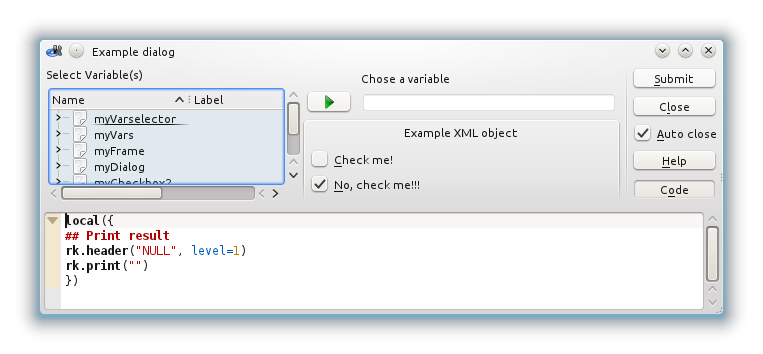
\includegraphics{./RKWard_vign_example_dialog_wcode.png}
 % RKWard_vign_example_dialog_wcode.png: 423x407 pixel, 99dpi, 10.85x10.44 cm, bb=0 0 308 296
\end{center}

Not bad for less than 20 short lines of code. This makes dialog design both very efficient and flexible:
Imagine you want to re-arrange the order of elements, or experiment with completely different tabbook layouts, all you need to
do is to change the \texttt{rk.XML.dialog()} call and run \texttt{rk.plugin.skeleton()} again (with \texttt{overwrite=TRUE}).
If you don't specify a directory explicitly, all will be written to a temporary directory. As seen in the example output,
the return value of \texttt{rk.plugin.skeleton()} is allways the root directory of the created plugin.

Looking at the attribute \texttt{xml=list(dialog=myDialog)}, we can assume that

\begin{enumerate}
	\item there's more than a \texttt{dialog} we can provide\\
		\textit{Further valid options are \texttt{wizard}, \texttt{logic} and \texttt{snippets}}
	\item there's more to define than just the \texttt{xml} of a plugin
		\textit{Further arguments include \texttt{js}, \texttt{pluginmap}, \texttt{rkh} and \texttt{components}, among others}
\end{enumerate}

Of course, this plugin doesn't really do anything useful. In fact, it doesn't matter how you treat the buttons and boxes, the R code below
won't change a bit, because we didn't provide any JavaScript code to deal with those events.

\subsection{Generating JavaScript code}
In contrast to what we've seen with the XML code, where objects are nested into others and the result is one big XML object, generated JavaScript code
is always a plain character string in the end. This is because it doesn't make much sense to treat a programming language otherwise, if you don't want
to lose its flexibility. But in between, existing objects will be re-used and new ones created as well. The best way to understand how \texttt{rkwarddev}
handles the JavaScript part is to think of it as a specialized \texttt{paste()}. Its special feature is that it understands the objects we're dealing
with, and depending on where they occur, knows what strings to make out of them.

Therefore, the most direct approach to get JavaScript into the plugin would to write it all by hand, paste it into a character object and give that to
\texttt{rk.plugin.skeleton()}. But again, \texttt{rkwarddev} offers some helpful tools.

\subsubsection{Defining variables}
We just created the XML dialog, which in turn of course includes all the elements (and their IDs) we need to care about. Or the other way round:
For each element in the dialog it is pretty safe to assume that it should have \textit{some} effect on the outcome. So for a start, \texttt{rkwarddev}
can ''scan`` the dialog object\footnote{In fact, \texttt{rk.JS.scan()} is not limited to R objects but can also read XML files.},
collect all relevant IDs and define them as JavaScript variables automatically. Try this for a demonstration:

	\begin{Schunk}
		\begin{Sinput}
> cat(rk.JS.scan(myDialog))
		\end{Sinput}
		\begin{Soutput}
  var vrslChosvrbl = getValue("vrsl_Chosvrbl");
  var chcCheckme = getValue("chc_Checkme");
  var chcNocheckm = getValue("chc_Nocheckm");
		\end{Soutput}
	\end{Schunk}

Notice that only the varslot and both checkboxes show up -- \texttt{rk.JS.scan()} distinguishes between relevant and irrelevant IDs, e.\,g. a
row or column is no GUI element of interest here. By the way, if you defined the frame as \texttt{checkable=TRUE}, its ID would be
extracted as well.\footnote{There is also a related function called \texttt{rk.JS.saveobj()}, which scans for \texttt{<saveobject>} nodes and
does not only define the neccessary variables, but also generates the full JavaScript code snippet for the \texttt{printout()} function,
to effectively save result objects to workspace.}

You might also notice that the JavaScript variable names differ from the XML IDs. For once, that way they're harder to confuse with each other,
and there's also some conventions which characters are allowed. But to cut things short, we don't have to worry about the variable names,
just like we didn't have to care about the XML IDs before. We don't even have to call \texttt{rk.JS.scan()} ourselves, as
\texttt{rk.plugin.skeleton()} will do so where appropriate, if the option \texttt{scan} includes \texttt{"var"}, which by default is the case.

This means, once more we can concentrate on what the plugin shall actually do, perhaps some calculation of a kind.

\subsubsection{Shortcut functions}
The common task here is to check for certain dialog events (like unchecking the checkbox labelled ''foo``), and then generate the according
\texttt{R} code (like \texttt{foo=FALSE}). The question remains, if we don't know the actual variable names, how can we check for events
of certain dialog elements in the JavaScript code? The answer to that is: We generate the code using \texttt{rkwarddev}'s special
JavaScripting functions and paste it with \texttt{rk.paste.JS()}. That way, we can use the created XML objects once again, as reference
to which element we actually mean.

\paragraph{echo()}
The JavaScript equivalent to \texttt{paste()} is \texttt{echo()}, with a slightly different
syntax: Concatenation is not done by commas, but by the plus sign, and the line must end with a semicolon. This is an example why it might be
nice to not need to switch between languages back and forth any more. So \texttt{rkwarddev} has an \texttt{R} function called \texttt{echo()},
which translates \texttt{paste()}-like arguments into an equivalent JavaScript call:

	\begin{Schunk}
		\begin{Sinput}
> echo("# Value of the checkbox is: ", myCheckbox, "\n")
		\end{Sinput}
		\begin{Soutput}
[1] "echo(\"# Value of the checkbox is: \" + chcCheckme + "\n");"
		\end{Soutput}
	\end{Schunk}

If this JavaScript code line was used, it would simply add a comment regarding the checkbox value to the \texttt{R} code,
including a newline.

\paragraph{ite()}
Now we know how to paste JavaScript code which echoes \texttt{R} code. What we definitely need at some point is \texttt{if()} conditions. For
that, \texttt{rkwarddev} offers \texttt{ite()}. The function takes up to three arguments: One ''if`` condition, one ''then`` action, and optionally
one ''else`` action. But actually, neither will the ''if`` condition be evaluated, nor will any of the actions be taken. The arguments just
define what should be \textit{pasted} at which part if the conditional statement:

	\begin{Schunk}
		\begin{Sinput}
> ite("foo", "bar", "baz")
		\end{Sinput}
		\begin{Soutput}
  if(foo) {
    bar
  } else {
    baz
  }
		\end{Soutput}
	\end{Schunk}

However, in contrast to \texttt{echo()}, what \texttt{ite()} returns is not a character string, but similar to what we've seen with the XML
functions a special JavaScript object. Amongst other things, this is useful to again generate readable code, e.\,g. nested conditions:

	\begin{Schunk}
		\begin{Sinput}
> ite(myCheckbox,
+   ite(myVars,
+     echo("result <- ", myVars, "\n"),
+     echo("# huh?\n")
+   ),
+   ite(myCheckbox2,
+     echo("## ouch!\n")
+   )
+ )
		\end{Sinput}
		\begin{Soutput}
  if(chcCheckme) {
    if(vrslChosvrbl) {
      echo("result <- " + vrslChosvrbl + "\n");
    } else {
      echo("# huh?\n");
    }
  } else if(chcNocheckm) {
    echo("## ouch!\n");
  } else {}
		\end{Soutput}
	\end{Schunk}

To finally use this object in the plugin, it must be evaluated and transformed into a character string.

\paragraph{rk.paste.JS()}
This is where \texttt{rk.paste.JS()} comes into play:

	\begin{Schunk}
		\begin{Sinput}
> myCalculation <- rk.paste.JS(
+   ite(myCheckbox,
+     ite(myVars,
+       echo("result <- ", myVars, "\n"),
+       echo("# huh?\n")
+     ),
+     ite(myCheckbox2,
+       echo("## ouch!\n")
+     )
+   )
+ )
+ rk.plugin.skeleton(
+   about="Example plugin",
+   xml=list(dialog=myDialog),
+   js=list(calculate=myCalculation),
+   load=TRUE,
+   show=TRUE,
+   overwrite=TRUE
+ )
		\end{Sinput}
		\begin{Soutput}
For filenames 'Example plugin' was renamed to 'Exampleplugin'.
For filenames 'Example plugin' was renamed to 'Exampleplugin'.
For filenames 'Example plugin' was renamed to 'Exampleplugin'.
For filenames 'Example plugin' was renamed to 'Exampleplugin'.
For filenames 'Example plugin' was renamed to 'Exampleplugin'.
[1] "/tmp/Rtmp9gdThb/Exampleplugin"
		\end{Soutput}
	\end{Schunk}

Now the plugin actually changes the generated code if you select an object from the workspace and toggle the checkboxes:

\begin{center}
 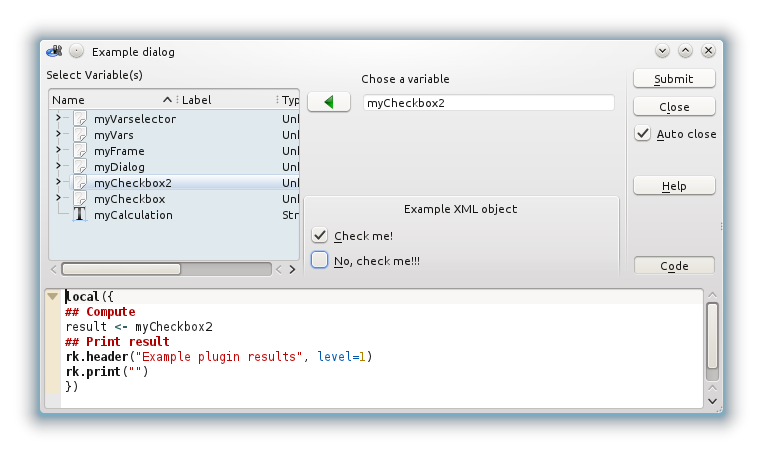
\includegraphics{./RKWard_vign_example_dialog_wcode_JS.png}
 % RKWard_vign_example_dialog_wcode_JS.png: 763x453 pixel, 99dpi, 19.57x11.62 cm, bb=0 0 555 329
\end{center}

% \subsection{The whole is more than the sum of its parts}
% 
% 
% 
% 	\begin{Schunk}
% 		\begin{Sinput}
% s
% 		\end{Sinput}
% 		\begin{Soutput}
% s
% 		\end{Soutput}
% 	\end{Schunk}

%  \begin{Schunk}
%  	\begin{Sinput}
%  	\end{Sinput}
%  	\begin{Soutput}
%  	\end{Soutput}
%  \end{Schunk}

%  \bibliographystyle{apacite}
%  \addcontentsline{toc}{chapter}{\bibname}
%  \bibliography{rkwarddev_lit}

\end{document}
